\chapter{Metric Spaces and Topology}

We initiate this chapter with a brief discussion of key mathematical concepts and motivate how they can be generalized to address important challenges.
We assume that the intended reader has experience with the real numbers, convergent sequences, and continuous functions.
Specifically, the reader should be familiar with the following notions.
\begin{itemize}
\item \textbf{Convergence:}
Suppose $x_1, x_2, \ldots$ is a sequence of real numbers.
This sequence converges to a point $x$ if, for any $\epsilon > 0$, there exists a number $N$ such that $| x_n - x | < \epsilon$ for all $n > N$.
\item \textbf{Continuity:}
Suppose $f : \RealNumbers \mapsto \RealNumbers$ is a real-valued function over the real numbers.
This function is continuous at $x_0$ if, for any $\epsilon > 0$, there exists a $\delta > 0$ such that $| f(x) - f(x_0) | < \epsilon$ for all $x \in \RealNumbers$ satisfying $|x - x_0| < \delta$.
\end{itemize}
One scenario where convergence plays an important role is in the design of iterative methods applied to optimization.
Therein, convergence properties can ensure that the iterative process leads to a well-defined answer.
Likewise, continuity is a cornerstone of calculus, differential equations, and probability.
These related concepts give rise to many practical mathematical tools like gradient descent and Newton's method.

The definitions above are empowering when dealing with the real numbers.
Yet, we are interested in exploring spaces that contain objects such as vectors, time series, images, arrays of data, polynomials, matrices, and functions.
This brings up an important question: How can we extend the notions of convergence and continuity to more general spaces?
Answering this question is key in better understanding the structure of abstract spaces and, also, in designing algorithms and iterative methods attuned to a rich class of problems.

A first step in developing a more powerful theory is to identify what makes these definitions work for the real numbers.
Based on the insights we gain from familiar examples, we can then extract key attributes and build intuition on how we can define similar concepts for abstract spaces.
We begin with pertinent questions.
First off, what are the real numbers and why do we use them all the time, as opposed to, say, the rational numbers?
Second, in the definition of convergence above, we need to know the limit of the sequence to show convergence.
However, when we design an iterative algorithm, we most likely do not know its limit; else we would not need to use an iteration process to get there.
Is there a notion of convergent sequence for which we do not need to pocess an explicit characterization of its limit beforehand?
Interestingly, both definitions rely on proximity, respectively $|x_n - x|$ and $|f(x) - f(x_0)|$.
We have a pretty good grasp of the distance between two points on the real line.
How can we define the distance between two points in more general setting?
These are the questions we seek to address below, in the hope of leveraging our familiarity with real numbers into understanding more general spaces.


\section{Metric Spaces}

From an applied perspective, the quintessential way to construct a topology on a space is to define the open sets in terms of a metric.
This approach underlies our intuitive understanding of open and closed sets on the real line.
Generally speaking, a metric captures the notion of a distance between two elements of a set.
Topologies that are defined through metrics possess a number of properties that make them suitable for analysis.
Identifying these common properties permits the unified treatment of different spaces that are useful in solving practical problems.
To gain better insight into metric spaces, we review the notion of a metric and we introduce a formal definition for topology.

\index{metric space}
A \textbf{metric space} is a set with a well-defined \emph{distance} between any two elements.
In some sense, such a space abstracts a few basic properties of Euclidean space.
Formally, a metric space $(X,d)$ is a set $X$ and a function $d$ called a metric.
The function $d(\cdot, \cdot)$ must fulfill the following properties.

\begin{definition}
A \defn{metric space}{metric} on a set $X$ is a function
\begin{equation*}
d \colon X \times X \rightarrow \RealNumbers
\end{equation*}
that satisfies the following properties,
\begin{enumerate}
\item $d(x,y) \geq 0 \quad \forall x, y \in X$; equality holds if and only if $x = y$
\item $d(x,y) = d(y,x) \quad \forall x, y \in X$
\item $d(x,y) + d(y,z) \geq d(x,z) \quad \forall x, y, z \in X$.
\end{enumerate}
\end{definition}

\begin{example}
The collection of real numbers equipped with the metric of absolute distance, $d(x,y) = |x-y|$, defines the standard metric space for the real numbers $\RealNumbers$.
\end{example}

\begin{example}
The set of vectors in $\RealNumbers^n$ can also be endowed with a metric.
Suppoe $\vecnot{x} = (x_1, \ldots, x_n)$ and $\vecnot{y} = (y_1, \ldots, y_n)$ are elements in $\RealNumbers^n$.
The \defn{metric space}{Euclidean metric} $d$ on $\RealNumbers^n$ is defined by
\begin{equation*}
d \left( \vecnot{x}, \vecnot{y} \right)
= \sqrt{ (x_1 - y_1)^2 + \cdots + (x_n - y_n)^2 }.
\end{equation*}
As implied by its name, the function $d(\cdot, \cdot)$ given above possesses all the properties of a metric.
\end{example}

It may be beneficial to also look at metrics that are less common.
The following two problems introduce alternate distances between points.

\begin{problem}
Let $\vecnot{x} = (x_1, \ldots, x_n), \vecnot{y} = (y_1, \ldots, y_n) \in \RealNumbers^n$ and consider the function $\rho$ given by
\begin{equation*}
\rho \left( \vecnot{x}, \vecnot{y} \right)
= \max \left\{ |x_1 - y_1|, \ldots, |x_n - y_n| \right\}.
\end{equation*}
Show that $\rho$ is a metric.
\end{problem}

\begin{problem} \label{problem:StandardBoundedMetric}
Let $X$ be a metric space with metric $d$.
Define $\bar{d}  \colon X \times X \rightarrow \RealNumbers$ by
\begin{equation*}
\bar{d} (x, y)
= \min \left\{ d (x, y), 1 \right\}.
\end{equation*}
Show that $\bar{d}$ is also a metric.
\end{problem}


\subsection{Convergence}

Let $(X,d)$ be a metric space.
Then, elements of $X$ are called \defn{metric space}{points} and the number $d(x,y)$ is called the \defn{metric space}{distance} between $x$ and $y$.
Let $\epsilon > 0$ and consider the set $B_d(x,\epsilon) = \left\{ y \in X | d(x,y) < \epsilon \right\}$.
This set is called the \defn{metric space}{$d$-open ball} (or open ball) of radius $\epsilon$ centered at $x$.

\begin{problem}
Suppose $a \in B_d(x, \epsilon)$ with $\epsilon > 0$.
Show that there exists a $d$-open ball centered at $a$ of radius $\delta$, say $B_d(a, \delta)$, that is contained in $B_d(x, \epsilon)$.
\end{problem}

One of the main benefits of having a metric is that it provides some notion of ``closeness'' between points in a set.
This allows one to discuss limits, convergence, open sets, and closed sets.

\begin{definition}
A \defn{metric space}{sequence} of elements from a set $X$ is an infinite list $x_1,x_2,\ldots$ where $x_i \in X$ for all $i\in \mathbb{N}$.
Formally, a sequence is equivalent to a function $f \colon \mathbb{N} \rightarrow X$ where $x_i = f(i)$ for all $i\in \mathbb{N}$.
\end{definition}

\begin{definition}
\label{definition_metspace_converge}
Consider a sequence $x_1, x_2, \ldots$ of points in a metric space $(X,d)$.
We say that $x_n$ \defn{metric space}{converges} to $x\in X$ (denoted by $x_n \to x$)  if, for any $\epsilon >0$, there is natural number $N$ such that $d(x,x_n) < \epsilon$ for all $n>N$.
\end{definition}

\begin{problem}
For a sequence $x_n$, show that $x_n \to a$ and $x_n \to b$ implies $a=b$.
\end{problem}

\begin{definition}
A sequence $x_1,x_2,\ldots$ in $(X,d)$ is a \defn{metric space}{Cauchy sequence} if, for any $\epsilon >0$, there is a natural number $N$ (depending on $\epsilon$) such that, for all $m,n > N$,
\begin{equation*}
d \left( x_m, x_n \right) < \epsilon.
\end{equation*}
\end{definition}



\begin{theorem}
Every convergent sequence is a Cauchy sequence.
\end{theorem}
\begin{proof}
Since $x_1,x_2,\ldots$ converges to some $x$, there is an $N$, for any $\epsilon>0$, such that $d(x,x_n)<\epsilon /2$ for all $n>N$.
The triangle inequality for $d(x_m,x_n)$ shows that, for all $m,n>N$,
\[ d(x_m,x_n)\leq d(x_m,x) + d(x,x_n) \leq \epsilon/2 + \epsilon/2 = \epsilon. \]
Therefore, $x_1,x_2,\ldots$ is a Cauchy sequence.
\end{proof}

\begin{example}
Let $(X,d)$ be the metric space  of rational numbers defined by $X=\mathbb{Q}$ and $d(x,y)=|x-y|$.
The sequence $x_1 = 2$, $x_{n+1} = \frac{1}{2}x_n + \frac{1}{x_n}$ satisfies $x_n \in \mathbb{Q} $ and, using $x_{n+1} - \sqrt{2} = \frac{1}{2x_n}(x_n-\sqrt{2})^2$, one can show it is Cauchy. But, it does not converge in $(X,d)$ because its limit point is the irrational number $\sqrt{2} \notin \mathbb{Q}$.
\end{example}

%\begin{example}
%Let $(X,d)$ be the metric space  of rational numbers defined by $X=\mathbb{Q}$ and $d(x,y)=|x-y|$.
%The sequence $x_n = \left( 1 + \frac{1}{n} \right)^n \in \mathbb{Q} $ is Cauchy but it does not converge in $(X,d)$ because its limit point is the real number $e \notin \mathbb{Q}$.
%\end{example}

\subsection{Metric Topology}

\begin{definition}
\label{definition:metspace_dopen}
Let $W$ be a subset of a metric space $(X,d)$.
The set $W$ is called \defn{metric space}{open} if, for every $w\in W$, there is an $\epsilon>0$ such that $B_d (w,\epsilon) \subseteq W$.
\end{definition}

\begin{theorem}
\label{theorem:d_open_closure}
For any metric space $(X,d)$,
\begin{enumerate}
\item $\emptyset$ and $X$ are open
\item any union of open sets is open
\item any finite intersection of open sets is open
\end{enumerate}
\end{theorem}
\begin{proof}
This proof is left as an exercise for the reader.
\end{proof}

One might be curious why only finite intersections are allowed in Theorem~\ref{theorem:d_open_closure}.
The following example highlights the problem with allowing infinite intersections.
\begin{example}
Let $I_n = \left(-\frac{1}{n},\frac{1}{n} \right) \subset \RealNumbers$, for $n\in \mathbb{N}$, be a sequence of open real intervals.
The infinite intersection
\[ \bigcap_{n\in \mathbb{N}} I_n = \{ x\in \RealNumbers | \forall n\in \mathbb{N}, x\in I_n \} = \{0 \}. \]
But, it is easy to verify that $\{ 0 \}$ is not an open set.
\end{example}

\begin{definition}
A subset $W$ of a metric space $(X,d)$ is \defn{metric space}{closed} if its complement $W^c = X-W$ is open.
\end{definition}

\begin{corollary}
For any metric space $(X,d)$,
\begin{enumerate}
\item $\emptyset$ and $X$ are closed
\item any intersection of closed sets is closed
\item any finite union of closed sets is closed
\end{enumerate}
\end{corollary}
\begin{proof}[Sketch of proof]
Using the definition of closed, one can apply De Morgan's Laws to Theorem~\ref{theorem:d_open_closure} verify this result.
\end{proof}

Actually, the sets $\emptyset$ and $X$ are both open and closed.
Such sets are called \textbf{clopen}.
For a non-trivial example, consider the standard metric space of rational numbers and choose $W = \{x\in \mathbb{Q}\,|\, x< \sqrt{2}\}$.
This set is open because, for all $x\in W$, we have $B(x,\sqrt{2}-x)\subseteq W$.
Since $\sqrt{2}\notin \mathbb{Q}$, it follows that $U = \{x\in \mathbb{Q}\,|\, x\geq \sqrt{2}\}=\{x\in \mathbb{Q}\,|\, x> \sqrt{2}\}$ which is open by the same argument.
But $\Complement{U} = W$, so $W$ is also closed.

\begin{definition}
For any metric space $(X,d)$ and subset $W \subseteq X$, a point $x\in X$ is a \defn{metric space}{limit point} of $W$ if there is a sequence $w_1,w_2,\ldots\in W \setminus \{ x \}$ of distinct elements that converges to $x$.
Equivalently, $x$ is a limit point of $W$ if, for all $\delta >0$, the set $\{ w\in W | d(x,w)<\delta \}$ contains some point besides $x$.
\end{definition}

\begin{problem}
Prove that the two definitions of a limit point are equivalent.
\end{problem}

By this definition (which is standard), an \defn{metric space}{isolated point} $w\in W$ is not a limit point because there is no sequence of distinct elements that converges to it.
Instead, for any sequence that converges to an isolated point $w$, there must be an $N\in \mathbb{N}$ such that $w_n = w$ for all $n>N$. 

\begin{theorem}
For any metric space $(X,d)$, a subset $W \subseteq X$ is closed if and only if it contains all of its limit points.
\end{theorem}

\begin{proof}
Assume $W$ is closed and suppose $x \notin W$ (i.e., $x \in W^c$) is a limit point of $W$.
Since $W^c$ is open, there is a $\delta > 0$ such that $B(x,\delta) \subseteq W^c$ and no sequence in $W$ can approach $x$. This contradicts the supposition that $x \notin W$ is a limit point and implies all limit points must be in $W$.
On the other hand, if $W$ contains all its limit points, then no $x \notin W$ (i.e., $x\in W^c$) can be a limit point.
Negating the second definition of a limit point and applying it to any $x \in W^c$, we see that there is a $\delta > 0$ such that $\{ w\in W | d(x,w)<\delta \}$ is empty.
Thus, $B_d (x,\delta) \subseteq W^c$ and this implies that $W^c$ is open.
Thus, $W$ is closed.
\end{proof}

It follows that, for a closed subset $W \subseteq X$, any sequence $w_n \in W$ that converges must converge to a point $w \in W$.

\begin{definition}
For any metric space $(X,d)$ and subset $W \subseteq X$, a point $w\in W$ is in the \defn{metric space}{interior} of $W$ if and only if there is a $\delta >0$ such that, for all $x\in X$ with $d(x,w)<\delta$, it follows that $x\in W$.
\end{definition}

\begin{problem}
Prove that the interior of a set is open.
\end{problem}

\begin{definition}
For any metric space $(X,d)$ and subset $W \subseteq X$, a point $x\in X$ is in the \defn{metric space}{closure} of $W$ if and only if, for all $\delta >0$, there is a $w\in W$ such that $d(x,w)<\delta$.
\end{definition}

\begin{problem}
Prove that the closure of a set contains all its limit points and, thus, is open.
\end{problem}

The interior of $A$ is denoted by $\Interior{A}$ and the closure of $A$ is denoted by $\Closure{A}$.
%Using Definition~\ref{definition:metspace_dopen}, it is easy to verify that $\Interior{A}$ is open.
%The definition of the closure of $W$ shows that it contains all of its limit points and, thus, is closed.
%Thus, $\Closure{A}$ is closed because a subset of a metric space is closed if and only if it contains all of its limit points.
The \defn{metric space}{boundary} $\partial A$ of a set $A$ is defined by $\partial A \triangleq \Closure{A} \setminus \Interior{A}$.

\subsection{Continuity}

Let $f \colon X \rightarrow Y$ be a function between the metric spaces $(X,d_X)$ and $(Y,d_Y)$.
\begin{definition}
The function $f$ is \defn{metric space}{continuous} at $x_0$ if, for any $\epsilon> 0$, there exists a $\delta >0$ such that, for all $x\in X$ satisfying $d_X(x_0,x)< \delta$, 
\[ d_Y \left( f(x_0),f(x) \right) < \epsilon .\]
In precise mathematical notation, one has
\begin{equation*}
\begin{split}
&(\forall \, \epsilon >0) ( \exists \, \delta >0)(\forall \, x \in \{x'\in X\,|\,d_X (x_0,x')<\delta\}),  \, d_Y \left( f(x_0),f(x) \right) < \epsilon .
\end{split}
\end{equation*}
\end{definition}

\begin{theorem} \label{thm:cont_fun_limit}
If $f$ is continuous at $x_0$, then $f(x_n) \to f(x_0)$ for all sequences $x_1,x_2,\ldots \in X$ such that $x_n \to x_0$.
Conversely, if $f(x_n) \to f(x_0)$ for all sequences $x_1,x_2,\ldots  \in X$ such that $x_n \to x_0$, then $f$ is continuous at $x_0$.
% if and only if  $f(x_n) \to f(x_0)$ for all sequences $x_1,x_2,\ldots \in X$ such that $x_n \to x_0$. 
\end{theorem}
\begin{proof}
If $f$ is continuous at $x_0$, then, for any $\epsilon > 0$, there is a $\delta >0$ such that $d_Y (f(x_0),f(x)) < \epsilon$ if $d_X (x_0,x) < \delta$.
If $x_n \to x_0$, then there is an $N\in \mathbb{N}$ such that $d_X (x_n,x_0) < \delta$ for all $n>N$.
Thus, $d_Y (f(x_0),f(x_n)) < \epsilon$ for all $n>N$ and $f(x_n) \to f(x_0)$.

For the converse, we show the contrapositive.
If $f$ is not continuous at $x_0$, then there exists an $\epsilon >0$ such that, for all $\delta >0$, there is an $x\in X$ with $d_X (x_0,x) < \delta$ and $d_Y (f(x_0),f(x))\geq \epsilon$.
For this $\epsilon$ and any positive sequence $\delta_n \to 0$, let $x_n$ be the promised $x$.
Then, $x_n \to x_0$ because $d_X (x_0,x_n)<\delta_n \to 0$ but $d_Y (f(x_0),f(x_n))\geq \epsilon$.
Thus, $f(x_n)$ does not converge to $f(x_0)$ for some sequence where $x_n \to x_0$.
\end{proof}

\begin{definition}
\boldmath
The \defn{metric space}{limit}~\textbf{of $f$ at $x_0$},
\unboldmath
$\lim_{x \to x_0} f(x)$, exists and equals $f(x_0)$ if $f(x_n) \to f(x_0)$ for all sequences $x_n \in X$ such that $x_n \to x_0$.
Thus, Theorem~\ref{thm:cont_fun_limit} implies that the limit of $f$ exists at $x_0$ if and only if $f$ is continuous at $x_0$.
\end{definition}

\begin{definition}
The function $f$ is called \defn{metric space}{continuous} if, for all $x_0 \in X$, it is continuous at $x_0$.
In precise mathematical notation, one has
\begin{equation*}
\begin{split}
(\forall \, x_0 \in X) & (\forall \, \epsilon >0) ( \exists \, \delta >0) \\ & (\forall \, x \in \{x'\in X\,|\,d_X (x_0,x')<\delta\}), \,
  d_Y \left( f(x_0),f(x) \right) < \epsilon .
\end{split}
\end{equation*}
\end{definition}

\begin{definition}
The function $f$ is called \defn{metric space}{uniformly continuous} if it is continuous and, for all $\epsilon > 0$, the $\delta >0$ can be chosen independently of $x_0$.
In precise mathematical notation, one has
\begin{equation*}
\begin{split}
(\forall \, \epsilon >0)  & ( \exists \, \delta >0) (\forall \, x_0 \in X) \\ & (\forall \, x \in \{x'\in X\,|\,d_X (x_0,x')<\delta\}), \,
  d_Y \left( f(x_0),f(x) \right) < \epsilon .
\end{split}
\end{equation*}
\end{definition}

\begin{definition}
A function $f  \colon X \rightarrow Y$ is called \defn{metric space}{Lipschitz continuous} on $A \subseteq X$ if there is a constant $L \in \RealNumbers$ such that $d_Y (f(x),f(y)) \leq L d_X (x,y)$ for all $x,y\in A$.
\end{definition}

Let $f_A$ denote the \textbf{restriction} of $f$ to $A\subseteq X$ defined by $f_A \colon A \to Y$ with $f_A (x) = f(x)$ for all $x\in A$.
It is easy to verify that, if $f$ is Lipschitz continuous on $A$, then $f_A$ is uniformly continuous.

\begin{problem}
Let $(X,d)$ be a metric space and define $f: X \to \mathbb{R}$ by $f(x)=d(x,x_0)$ for some fixed $x_0 \in X$.
Show that $f$ is Lipschitz continuous with $L=1$.
\end{problem}

% d(x,x_0) <= d(x,y) + d(y,x_0)
% d(y,x_0) <= d(x,y) + d(x,x_0)
% |f(x)-f(y)| <= d(x,y)

\subsection{Completeness}
\label{sec:metspace_complete}
Suppose $(X,d)$ is a metric space.
From Definition~\ref{definition_metspace_converge}, we know that a sequence $x_1, x_2, \ldots$ of points in $X$ converges to $x \in X$ if, for every $\delta >0$, there exists an integer $N$ such that $d(x_i,x)<\delta$ for all $i \geq N$.
%if for every neighborhood $A$ of $x$ there exists a positive integer $N$ such that $x_i \in A$ for all $i \geq N$.

\begin{figure}[ht]
\begin{center}
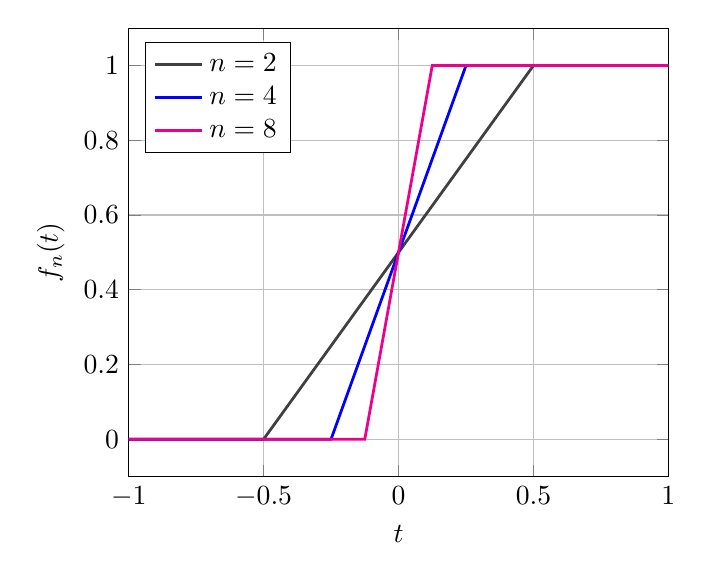
\begin{tikzpicture}
\begin{axis}[
    %title={Continuous Functions},
    xlabel={$t$},
    xmin=-1, xmax=1,
    xmajorgrids,
    ylabel={$f_n(t)$},
    ymajorgrids,
    legend pos=north west]
\addplot[darkgray,line width=1pt] coordinates {
    (-1,0) (-0.5,0) (0.5,1) (1,1)};
\addlegendentry{$n = 2$}

\addplot[blue,line width=1pt] coordinates {
    (-1,0) (-0.25,0) (0.25,1) (1,1)};
\addlegendentry{$n = 4$}

\addplot[magenta,line width=1pt] coordinates {
    (-1,0) (-0.125,0) (0.125,1) (1,1)};
\addlegendentry{$n = 8$}
\end{axis}
\end{tikzpicture}
\vspace{-8mm}
\end{center}
\caption{The sequence of continuous functions in Example~\ref{example:ContinuousFunctionsCauchy} satisfies the Cauchy criterion.
But, it does not converge to a continuous function in $C[-1,1]$.}
\end{figure}

It is possible for a sequence in a metric space $X$ to satisfy the Cauchy criterion, but not to converge in $X$.

\begin{example}
\label{example:ContinuousFunctionsCauchy}
Let $X=C[-1,1]$ be the space of continuous functions that map $[-1,1]$ to $\mathbb{R}$ and satisfy $\left\| f \right\|_2 < \infty$, where $\left\| f \right\|_2$ denotes the $L^2$ norm
\begin{equation*}
\left\| f \right\|_2 \triangleq \left( \int_{-1}^1 |f(t)|^2 dt \right)^{\frac{1}{2}}.
\end{equation*}
This set forms a metric space $(X,d)$ when equipped with the distance
\[ d(f, g) \triangleq \left\| f - g \right\|_2
= \left( \int_{-1}^1 |f(t) - g(t)|^2 dt \right)^{\frac{1}{2}}. \]
Consider the sequence of functions $f_n(t)$ given by
\begin{equation*}
f_n(t) \triangleq \left\{ \begin{array}{ll}
0 & t \in \left[ -1, -\frac{1}{n} \right] \\
\frac{nt}{2} + \frac{1}{2} & t \in \left( -\frac{1}{n}, \frac{1}{n} \right) \\
1 & t \in \left[ \frac{1}{n}, 1 \right].
\end{array} \right\}
\end{equation*}

Assuming that $m \geq n$, a bit of calculus shows that
\begin{equation*}
d(f_n, f_m) = \left\| f_n(t) - f_m(t) \right\|_2
= \left( \int_{-1}^1 |f_n(t) - f_m(t)|^2 dt \right)^{\frac{1}{2}}
= \frac{(m-n)^2}{6m^2n}.
\end{equation*}
Since $m\geq n$, this distance is upper bounded by $\frac{1}{6n}$ and the sequence satisfies the Cauchy criterion.
But, it does not converge to a continuous function in $C[-1,1]$.
\end{example}

\begin{definition}
A metric space $(X,d)$ is said to be \defn{metric space}{complete} if every Cauchy sequence in $(X,d)$ converges to a limit $x \in X$.
\end{definition}

The standard metric space of real numbers with absolute distance is a complete metric space.
This fact and other foundational properties of the real numbers can be derived formally using the techniques described below.
However, a formal construction of the real numbers will not be provided in these notes.

%\begin{example}
%Any closed subset of $\mathbb{R}^n$ (or $\mathbb{C}^n$) is complete.
%\end{example}

\begin{example}
Consider the sequence $x_1 = 2$, $x_{n+1} = \frac{1}{2}x_n + \frac{1}{x_n}$ and observe that $x_n \in \mathbb{Q}$ for all $n\in \mathbb{N}$.
We saw earlier that $x_n$ is a Cauchy sequence with limit point $\sqrt{2} \in \mathbb{R}$.
But, $\sqrt{2}$ is irrational and thus the rational numbers $\mathbb{Q}$ are not complete.
\end{example}

\begin{theorem}
A closed subset $A$ of a complete metric space $X$ is itself a complete metric space.
\end{theorem}
\begin{proof}
Any Cauchy sequence $x_1,x_2,\ldots \in A$ is also a Cauchy sequence in $X$.
This implies that $x_n \to x \in X$ and it follows that $x \in \Closure{A}$.
Since $A$ is closed, $x\in A$.
\end{proof}

\begin{definition}
An \defn{metric space}{isometry} is a mapping $\phi  \colon X \rightarrow Y$ between two metric spaces $(X,d_X)$ and $(Y,d_Y)$ that is distance preserving (i.e., it satisfies $d_X (x,x') = d_Y \left(\phi(x),\phi(x')\right)$ for all $x,x'\in X$).
\end{definition}

\begin{definition}
A subset $A$ of a metric space $(X,d)$ is \defn{metric space}{dense} in $X$ if every $x\in X$ is a limit point of the set $A$.
This is equivalent to its closure $\overline{A}$ being equal to $X$.
\end{definition}

\begin{definition}
The \defn{metric space}{completion} of a metric space $(X,d_X)$ consists of a complete metric space $(Y,d_Y)$ and an isometry $\phi  \colon X \rightarrow Y$ such that $\phi(X)$ is a dense subset of $Y$.
Moreover, the completion is unique up to isometry.
\end{definition}

\begin{example}
Consider the metric space $\mathbb{Q}$ of rational numbers equipped with the metric of absolute distance.
The completion of this metric space is $\RealNumbers$ because the isometry is given by the identity mapping and $\mathbb{Q}$ is a dense subset of $\RealNumbers$.
\end{example}

Cauchy sequences have many applications in analysis and signal processing.
For example, they can be used to construct the real numbers from the rational numbers.
In fact, the same approach is used to construct the completion of any metric space.

\begin{definition}
Two Cauchy sequences $x_1, x_2, \ldots$ and $y_1, y_2, \ldots$ are equivalent if, for every $\epsilon >0$, there exists an integer $N$ such that $d (x_k, y_k) \leq \epsilon$ for all $k \geq N$.
\end{definition}

\begin{example}
Let $\mathcal{C}(\mathbb{Q})$ denote the set of all Cauchy sequences $q_1, q_2, \ldots$ of rational numbers where $\sim$ represents the equivalence relation on this set defined above.
Then, the set of equivalence classes (or quotient set) $\mathcal{C}(\mathbb{Q}) / \! \sim$ is in one-to-one correspondence with the real numbers.
This construction is the standard completion of $\mathbb{Q}$.
Since every Cauchy sequence of rationals converges to a real number, the isometry is given by mapping each equivalence class to its limit point in $\RealNumbers$.
\end{example}

\begin{definition}
Let $A$ be a subset of a metric space $(X,d)$ and $f \colon X \rightarrow X$ be a function.
Then, $f$ is a \defn{metric space}{contraction} on $A$ if $f(A) \subseteq A$ and there exists a constant $\gamma < 1$ such that $d \left( f(x),f(y) \right) \leq \gamma  d(x,y)$ for all $x,y\in A$.
\end{definition}

Consider the following important results in applied mathematics: Picard's uniqueness theorem for differential equations, the implicit function theorem, and the existence of stationary optimal policies for Markov decision processes.
What do they have in common?
They each establish the existence and uniqueness of a function and have relatively simple proofs based on the contraction mapping theorem.

\begin{theorem}[Contraction Mapping Theorem]
Let $(X,d)$ be a complete metric space and $f$ be contraction on a closed subset $A \subseteq X$.
Then, $f$ has a unique fixed point $x^*$ in $A$ such that $f(x^*) = x^*$ and the sequence $x_{n+1} = f(x_n)$ converges to $x^*$ for any point $x_1 \in A$.  Moreover, $x_n$ satisfies the error bounds $d(x^*,x_n) \leq \gamma^{n-1} d(x^*,x_1)$ and $d(x^*,x_{n+1}) \leq d(x_n,x_{n+1})\gamma /(1-\gamma)$.
\end{theorem}
\begin{proof}
Suppose $f$ has two fixed points $y,z\in A$.
Then, $d(y,z) = d \left(f(y),f(z) \right) \leq \gamma  d(y,z)$ and $d(y,z) = 0$ because $\gamma \in [0,1)$.
This shows that $y=z$ and any two fixed points in $A$ must be identical.

Since $d(f(x_n),f(x_{n+1})) \leq \gamma d(x_n,x_{n+1})$, induction shows that $d(x_n,x_{n+1}) \leq \gamma^{n-1} d(x_1,x_2)$.
Using this, we can bound the distance $d(x_m,x_n)$ (for $m<n$) with
\begin{align*}
d(x_m,x_n)
& \leq d(x_m,x_{m+1}) + d(x_{m+1},x_n) \\
& \leq \sum_{i=m}^{n-1} d(x_i,x_{i+1}) 
 \leq \sum_{i=m}^{n-1} \gamma^{i-1} d(x_1,x_2) \\
& \leq \sum_{i=m}^\infty \gamma^{i-1} d(x_1,x_2) 
 \leq \frac{\gamma^{m-1}}{1-\gamma} d(x_1,x_2).
\end{align*}
The sequence $x_n$ is Cauchy because $d(x_m,x_n)$ can be made arbitrarily small (for all $n>m$) by increasing $m$.
As $(X,d)$ is complete, it follows that $x_n \to x^*$ for some $x^* \in X$.
Since $f$ is Lipschitz continuous, this implies that $x^* = \lim_n x_n = \lim_n f(x_n) = f(x^*)$ the unique fixed point of $f$ in $A$.

Arguments similar to the above can be used to prove the stated error bounds.
\end{proof}

\begin{figure}[t]
\centering
% This file was created by matlab2tikz v0.3.0.
% Copyright (c) 2008--2012, Nico Schlömer <nico.schloemer@gmail.com>
% All rights reserved.
% 
% The latest updates can be retrieved from
%   http://www.mathworks.com/matlabcentral/fileexchange/22022-matlab2tikz
% where you can also make suggestions and rate matlab2tikz.
% 
% 
% 
% defining custom colors
\definecolor{mycolor1}{rgb}{0,0.447,0.741}
\definecolor{mycolor2}{rgb}{0.85,0.325,0.098}
\definecolor{mycolor3}{rgb}{1,0,1}
\begin{tikzpicture}
\begin{axis}[%
width=3in,
height=2.5in,
every outer x axis line/.append style={darkgray!60!black},
every x tick label/.append style={font=\color{darkgray!60!black}},
grid=major,
xmin=0, xmax=1,
xlabel={$x_n$},
every outer y axis line/.append style={darkgray!60!black},
every y tick label/.append style={font=\color{darkgray!60!black}},
ymin=0, ymax=1,
ylabel={$x_{n+1}$}]
\addplot [
thick,
color=mycolor1,
solid,
forget plot
]
coordinates{
 (0,0)(0.01,0.01)(0.02,0.02)(0.03,0.03)(0.04,0.04)(0.05,0.05)(0.06,0.06)(0.07,0.07)(0.08,0.08)(0.09,0.09)(0.1,0.1)(0.11,0.11)(0.12,0.12)(0.13,0.13)(0.14,0.14)(0.15,0.15)(0.16,0.16)(0.17,0.17)(0.18,0.18)(0.19,0.19)(0.2,0.2)(0.21,0.21)(0.22,0.22)(0.23,0.23)(0.24,0.24)(0.25,0.25)(0.26,0.26)(0.27,0.27)(0.28,0.28)(0.29,0.29)(0.3,0.3)(0.31,0.31)(0.32,0.32)(0.33,0.33)(0.34,0.34)(0.35,0.35)(0.36,0.36)(0.37,0.37)(0.38,0.38)(0.39,0.39)(0.4,0.4)(0.41,0.41)(0.42,0.42)(0.43,0.43)(0.44,0.44)(0.45,0.45)(0.46,0.46)(0.47,0.47)(0.48,0.48)(0.49,0.49)(0.5,0.5)(0.51,0.51)(0.52,0.52)(0.53,0.53)(0.54,0.54)(0.55,0.55)(0.56,0.56)(0.57,0.57)(0.58,0.58)(0.59,0.59)(0.6,0.6)(0.61,0.61)(0.62,0.62)(0.63,0.63)(0.64,0.64)(0.65,0.65)(0.66,0.66)(0.67,0.67)(0.68,0.68)(0.69,0.69)(0.7,0.7)(0.71,0.71)(0.72,0.72)(0.73,0.73)(0.74,0.74)(0.75,0.75)(0.76,0.76)(0.77,0.77)(0.78,0.78)(0.79,0.79)(0.8,0.8)(0.81,0.81)(0.82,0.82)(0.83,0.83)(0.84,0.84)(0.85,0.85)(0.86,0.86)(0.87,0.87)(0.88,0.88)(0.89,0.89)(0.9,0.9)(0.91,0.91)(0.92,0.92)(0.93,0.93)(0.94,0.94)(0.95,0.95)(0.96,0.96)(0.97,0.97)(0.98,0.98)(0.99,0.99)(1,1) 
};
\addplot [
very thick,
color=red, %mycolor2,
solid,
forget plot
]
coordinates{
 (0,1)(0.01,0.999950000416665)(0.02,0.999800006666578)(0.03,0.999550033748988)(0.04,0.999200106660978)(0.05,0.998750260394966)(0.06,0.998200539935204)(0.07,0.99755100025328)(0.08,0.996801706302619)(0.09,0.995952733011994)(0.1,0.995004165278026)(0.11,0.993956097956697)(0.12,0.992808635853866)(0.13,0.991561893714788)(0.14,0.990215996212637)(0.15,0.988771077936042)(0.16,0.987227283375627)(0.17,0.985584766909561)(0.18,0.983843692788121)(0.19,0.98200423511727)(0.2,0.980066577841242)(0.21,0.978030914724148)(0.22,0.975897449330606)(0.23,0.973666395005375)(0.24,0.97133797485203)(0.25,0.968912421710645)(0.26,0.966389978134513)(0.27,0.963770896365891)(0.28,0.961055438310771)(0.29,0.958243875512697)(0.3,0.955336489125606)(0.31,0.952333569885713)(0.32,0.949235418082441)(0.33,0.946042343528387)(0.34,0.942754665528346)(0.35,0.939372712847379)(0.36,0.935896823677935)(0.37,0.932327345606034)(0.38,0.92866463557651)(0.39,0.924909059857313)(0.4,0.921060994002885)(0.41,0.917120822816605)(0.42,0.913088940312308)(0.43,0.908965749674885)(0.44,0.904751663219963)(0.45,0.900447102352677)(0.46,0.896052497525525)(0.47,0.891568288195329)(0.48,0.886994922779284)(0.49,0.882332858610121)(0.5,0.877582561890373)(0.51,0.872744507645751)(0.52,0.86781917967765)(0.53,0.862807070514761)(0.54,0.857708681363824)(0.55,0.852524522059506)(0.56,0.847255111013416)(0.57,0.841900975162269)(0.58,0.836462649915187)(0.59,0.830940679100164)(0.6,0.825335614909678)(0.61,0.819648017845479)(0.62,0.813878456662534)(0.63,0.808027508312152)(0.64,0.802095757884293)(0.65,0.796083798549056)(0.66,0.789992231497365)(0.67,0.783821665880849)(0.68,0.777572718750928)(0.69,0.771246014997107)(0.7,0.764842187284488)(0.71,0.758361875990508)(0.72,0.751805729140895)(0.73,0.74517440234487)(0.74,0.738468558729588)(0.75,0.731688868873821)(0.76,0.724836010740905)(0.77,0.717910669610943)(0.78,0.710913538012277)(0.79,0.703845315652236)(0.8,0.696706709347165)(0.81,0.689498432951747)(0.82,0.682221207287613)(0.83,0.674875760071267)(0.84,0.667462825841308)(0.85,0.659983145884982)(0.86,0.652437468164052)(0.87,0.644826547240001)(0.88,0.63715114419858)(0.89,0.629412026573697)(0.9,0.621609968270664)(0.91,0.613745749488812)(0.92,0.605820156643463)(0.93,0.597833982287298)(0.94,0.589788025031098)(0.95,0.581683089463883)(0.96,0.573519986072457)(0.97,0.565299531160354)(0.98,0.557022546766217)(0.99,0.548689860581588)(1,0.54030230586814) 
};
\addplot [
thick,
color=mycolor3,
dashed,
forget plot
]
coordinates{
 (0.2,0.2)(0.2,0.980066577841242)(0.980066577841242,0.980066577841242) 
};
\addplot [
thick,
color=mycolor3,
dashed,
forget plot
]
coordinates{
 (0.980066577841242,0.980066577841242)(0.980066577841242,0.556967252809642)(0.556967252809642,0.556967252809642) 
};
\addplot [
thick,
color=mycolor3,
dashed,
forget plot
]
coordinates{
 (0.556967252809642,0.556967252809642)(0.556967252809642,0.848862165658271)(0.848862165658271,0.848862165658271) 
};
\addplot [
thick,
color=mycolor3,
dashed,
forget plot
]
coordinates{
 (0.848862165658271,0.848862165658271)(0.848862165658271,0.660837551116615)(0.660837551116615,0.660837551116615) 
};
\addplot [
thick,
color=mycolor3,
dashed,
forget plot
]
coordinates{
 (0.660837551116615,0.660837551116615)(0.660837551116615,0.789478437766868)(0.789478437766868,0.789478437766868) 
};
\addplot [
thick,
color=mycolor3,
dashed,
forget plot
]
coordinates{
 (0.789478437766868,0.789478437766868)(0.789478437766868,0.704215713341993)(0.704215713341993,0.704215713341993) 
};
\addplot [
thick,
color=mycolor3,
dashed,
forget plot
]
coordinates{
 (0.704215713341993,0.704215713341993)(0.704215713341993,0.762119561760661)(0.762119561760661,0.762119561760661) 
};
\addplot [
thick,
color=mycolor3,
dashed,
forget plot
]
coordinates{
 (0.762119561760661,0.762119561760661)(0.762119561760661,0.723374172105571)(0.723374172105571,0.723374172105571) 
};
\addplot [
thick,
color=mycolor3,
dashed,
forget plot
]
coordinates{
 (0.723374172105571,0.723374172105571)(0.723374172105571,0.749576576331493)(0.749576576331493,0.749576576331493) 
};
\end{axis}
\end{tikzpicture}%
\vspace{-5mm}
\caption{\label{fig:cos_contract}Starting from $x_1 = 0.2$, the iteration in Example~\ref{exa:cos_contract} maps $x_n$ to $x_{n+1}= \cos(x_n)$.  The points are also connected to the slope-1 line to show the path.}
\end{figure}

\begin{example} \label{exa:cos_contract}
Consider the cosine function restricted to the subset $[0,1]\subseteq \RealNumbers$.
Since $\cos(x)$ is decreasing for $0 \leq x < \pi$, we have $\cos([0,1]) = [\cos(1),1]$ with $\cos(1) \approx 0.54$.
The mean value theorem of calculus also tells us that $\cos(y) - \cos(x) = \cos '(t) (y-x)$ for some $t\in [x,y]$.
Since $\cos '(t) = -\sin(t)$ and $\sin(t)$ is increasing on $[0,1]$, we find that $\sin([0,1]) = [0,\sin(1)]$ with $\sin(1) \approx 0.84$.

Taking the absolute value, shows that $| \cos(y) - \cos(x) | \leq 0.85 |y-x|$.
Therefore, $\cos(t)$ is a contraction on $[0,1]$ and the sequence $x_{n+1} = \cos(x_n)$ (e.g., see Figure~\ref{fig:cos_contract}) converges to the unique fixed point $x^* = \cos(x^*)$ for all $x_1 \in [0,1]$.
\end{example}

%\begin{example}
%Suppose the function $f \colon \RealNumbers \rightarrow \RealNumbers$ satisfies $|f(x)| \leq a |x|$ for all $x\in X$.
%If $X$ be a closed subset of the real numbers containing zero and $a\in[0,1)$, then $f$ is a contraction on $X$ and $x_{n+1} = f(x_n) \rightarrow 0$ for all $x_1 \in X$.
%\end{example}


\subsection{Compactness}
\label{sec:metspace_compact}

\begin{definition}
A metric space $(X,d)$ is \defn{metric space}{totally bounded} if, for any $\epsilon > 0$, there exists a finite set of $B_d (x,\epsilon)$ balls that cover (i.e., whose union equals) $X$.
\end{definition}

\begin{definition}
A metric space is \defn{metric space}{compact} if it is complete~and~totally~bounded.
\end{definition}

The closed interval $[0,1]\subset \RealNumbers$ is compact.
In fact, a subset of $\RealNumbers^n$ is compact if and only if it is closed and bounded.
On the other hand, the standard metric space of real numbers is not compact because it is not totally bounded.

\begin{theorem}
\label{thm:CompactClosedSubsetCompact}
A closed subset $A$ of a compact space $X$ is itself a compact space.
\end{theorem}

The following theorem highlights one of the main reasons that compact spaces are desirable in practice.

\begin{theorem}
Let $(X,d)$ be a compact metric space and $x_1,x_2,\ldots \in X$ be a sequence.
Then, there is a subsequence $x_{n_1},x_{n_2},\ldots$, defined by some increasing sequence $n_1,n_2,\ldots \in \mathbb{N}$, that converges.
\end{theorem}
\begin{proof}
We proceed by recursively constructing subsequences $z^{(k)}_n$ starting from $z^{(0)}_n = x_n$.
Since $X$ is totally bounded, let $C_k \subset X$ be the centers of a finite set of balls with radius $2^{-k}$ that cover $X$ (i.e., $\cup_{x\in C_k} B(x,2^{-k}) = X$).
Then, one of these balls (say centered at $x'$) must contain infinitely many elements in $z^{(k-1)}_n$ (i.e., $\exists x' \in C_k, \,|\{n\in \mathbb{N}\,|\,z^{(k-1)}_n \in B(x',2^{-k})\}|=\infty$).
Next, we extract the subsequence contained in this ball by choosing $z^{(k)}_n$ to be the subsequence of $z^{(k-1)}_n$ contained in $B(x',2^{-k})$.
From the triangle inequality, it follows that $d(y,y')<2(2^{-k})$ for all $y,y'\in B(x',2^{-k})$.
Thus, $d(z^{(k')}_m,z^{(k)}_n) < 2^{-k+1}$ for all $m>n\geq 1$ and $k'\geq k \geq 1$.

Let $I(k,n)$ be the index in the original sequence associated with $z^{(k)}_n$.
Since each stage only removes elements from the previous subsequence and relabels, it follows that $I(k+1,k+1) \geq I(k,k+1) > I(k,k)$.
This implies that the sequence $y_k = z^{(k)}_k = x_{I(k,k)}$ is a subsequence of $x_n$ and
$d(y_m,y_k) \leq 2^{-k+1}$ for all $m>k$ and $k\geq1$.
Thus, for any $\epsilon >0$, choosing $N = \lceil \log_2 \frac{1}{\epsilon} \rceil + 1$ shows that $y_k$ is a Cauchy sequence.
Since $X$ is complete, it follows that $y_k$ converges to some $y\in X$.
\iffalse
There is a subsequence that converges  if and only if there is an $x\in X$ such that, for all $\epsilon>0$, the ball $B(x,\epsilon)$ contains infinitely many elements in the sequence (i.e., $|\{n\in \mathbb{N}\,|\,x_n \in B(x,\epsilon)\}|=\infty$).
In this case, one can choose $n_1 < n_2 < \cdots$ so that $d(x,x_{n_j}) \! < \! \frac{1}{j}$ for all $j\in \mathbb{N}$ and, thus, the subsequence $x_{n_j}$ converges to $x$.

Suppose there is no convergent subsequence.
Then, for all $x\in X$, there is an $\epsilon >0$ such that $B(x,\epsilon)$ contains a finite number of elements in the sequence (i.e., $|\{n\in \mathbb{N}\,|\,x_n \in B(x,\epsilon)\}| \leq N<\infty$ ).
Since $X$ is totally bounded, we also find that, for any $\epsilon >0$, $X$ is covered by a finite number (say $M$) of balls with radius $\epsilon$.
But, for each $\epsilon >0$, this gives a contradiction because all the elements in the infinite sequence must fall into a finite number balls each containing finitely many elements.
By contradiction, this implies that there is a subsequence that converges.
\fi
%First, we suppose the sequence has no convergent subsequence.
%Then, we notice that the set $A = \{x_1,x_2,\ldots \}$ is closed because it contains all its limit points.
%Thus, it is compact by Theorem~\ref{thm:CompactClosedSubsetCompact}.
%Since any limit point of $A$ can be used to generate a convergent subsequnce, we must also conclude that $A$ has no limit points.
%This implies that there is an $\epsilon > 0$ such that infinitely balls around $x$'s does not cover $X$.
%Therefore, $X$ is not totally bounded and we have a contradiction.
\end{proof}

Functions from compact sets to the real numbers are very important in practice.
To keep the discussion self-contained, we first review the extreme values of sets of real numbers.
First, we must define the \defn{topology}{extended real numbers} $\overline{\RealNumbers}$ by augmenting the real numbers to include limit points for unbounded sequences $\overline{\RealNumbers} \triangleq \RealNumbers \cup \{ \infty,-\infty\}$.
Using the metric $d_{\overline{\RealNumbers}} (x,y) \triangleq |\frac{x}{1+|x|} - \frac{y}{1+|y|}|$, this set becomes a compact metric space.
The main difference from $\RealNumbers$ is that, for  $x_n \in \overline{\RealNumbers}$, the statement  $x_n \to \infty$ is well defined and equivalent to $\forall M>0, \, \exists N\in \mathbb{N}, \, \forall n>N, \, x_n > M$.
\begin{definition}
The \defn{set theory}{supremum} (or least upper bound) of $X\subseteq \RealNumbers$, denoted $\sup X$, is the smallest extended real number $M \in \overline{\RealNumbers}$ such that $x\leq M$ for all $x\in X$.
It is always well-defined and equals $-\infty$ if $X=\emptyset$.
\end{definition}

\begin{definition}
The \defn{set theory}{maximum} of $X\subseteq \RealNumbers$, denoted $\max X$, is the largest value achieved by the set.
It equals $\sup X$ if $\sup X \in X$ and is undefined otherwise.
\end{definition}

\begin{definition}
The \defn{set theory}{infimum} (or greatest lower bound) of $X\subseteq \RealNumbers$, denoted $\inf X$, is the largest extended real number $m \in \overline{\RealNumbers}$ such that $x\geq m$ for all $x\in X$.
It is always well-defined and equals $\infty$ if $X=\emptyset$.
\end{definition}

\begin{definition}
The \defn{set theory}{minimum} of $X\subseteq \RealNumbers$, denoted $\min X$, is the smallest value achieved by the set.
It equals $\inf X$ if $\inf X \in X$ and is undefined otherwise.
\end{definition}

\begin{lemma}
\label{lem:SupremumSequence}
Let $X$ be a set and $f \colon X\rightarrow \RealNumbers$ be a function from $X$ to the real numbers.
Let $M = \sup f(A)$ for some non-empty $A \subseteq X$.
Then, there exists a sequence $x_1,x_2,\ldots \in A$ such that $\lim_n f(x_n) = M$.
\end{lemma}
\begin{proof}
If $M=\infty$, then $f(A)$ has no finite upper bound and, for any $y\in \RealNumbers$, there exists an $x\in A$ such that $f(x)>y$.
In this case, we can let $x_1$ be any element of $A$ and $x_{n+1}$ be any element of $A$ such that $f(x_{n+1}) > f(x_n) + 1$.
In the metric space $(\overline{\RealNumbers},d_{\overline{\RealNumbers}})$, this implies that $d_{\overline{\RealNumbers}}(f(x_n),\infty) = |\frac{f(x_n)}{1+|f(x_n)|} - 1| \to 0$ and thus $f(x_n) \to \infty$.

If $M<\infty$, then $f(A)$ has a finite upper bound and, for any $\epsilon >0$, there is an $x$ such that $M-f(x)<\epsilon$.
Otherwise, one arrives at the contradiction $\sup f(A) < M$.
Therefore, we can construct the sequence $x_1,x_2,\ldots$ by choosing $x_n\in A$ to be any point that satisfies $M-f(x_n)\leq \frac{1}{n}$.
\end{proof}

\begin{theorem}
Let $X$ be a metric space and $f \colon X\rightarrow \RealNumbers$ be a continuous function from $X$ to the real numbers.
If $A$ is a compact subset of $X$, then there exists $x\in A$ such that $f(x)=\sup f(A)$ (i.e., $f$ achieves a maximum on $A$).
\end{theorem}
\begin{proof}
Using Lemma~\ref{lem:SupremumSequence}, one finds that there is a sequence $x_1,x_2,\ldots \in A$ such that $\lim_n f(x_n) = \sup f(A)$.
Since $A$ is compact, there must also be a subsequence $x_{n_1},x_{n_2},\ldots$ that converges.
As $A$ is closed, this subsequence must converge to some $x^* \in A$.
Finally, the continuity of $f$ shows that
\[\sup f(A) = \lim_n f(x_n) = \lim_k f(x_{n_k}) = f(\lim_k x_{n_k}) = f(x^*). \qedhere \]
\end{proof}

\begin{corollary}
Let $(X,d)$ be a metric space.
Then, a continuous function from a compact subset $A\subseteq X$ to the real numbers achieves a minimum on $A$.
\end{corollary}

\begin{theorem}
Any bounded non-decreasing sequence of real numbers converges to its supremum.
\end{theorem}
\begin{proof}
Let $x_1,x_2,\ldots \in \RealNumbers$ be a sequence satisfying $x_{n+1} \geq x_n$ and $x_n \leq M < \infty$ for all $n\in \mathbb{N}$.
Without loss of generality, we can choose the upper bound $M$ to be the supremum $\sup \{x_1,x_2,\ldots\}$.
Now, we will prove directly that $x_n \to M$.

First, we note that the definition of the supremum implies that $x_n \leq M$ for all $n\in \mathbb{N}$ and, for any $\epsilon >0$, there is an $N\in \mathbb{N}$ such that $x_N > M-\epsilon$.
Second, since $x_n$ is non-decreasing, this implies that $x_n > M-\epsilon$ for all $n>N$.
Third, since $x_n \leq M$ by definition, it follows that $|M - x_n| = M-x_n < \epsilon$ for all $n>N$.
Thus, the constructed $N$ satisfies all elements in the definition of $x_n \to M$.
%To prove this by contradiction, we suppose that $x_n$ does not converge to $M$.
%Since $x_n$ is non-decreasing, this implies that there is an $\epsilon > 0$ such that $M - x_n \geq \epsilon$ for all $n\in \mathbb{N}$.
%But, this result contradicts $\sup f(A) = M$.
%Therefore, the sequence converges to $M$.
\end{proof}


\begin{lemma} \label{lem:sum_convergence}
Let $y_n \in \RealNumbers$ be a real sequence and $x_n = \sum_{i=1}^n y_i$ be its sequence of partial sums.
Then, $\sum_{i=1}^\infty y_i \triangleq \lim_{n\to \infty} x_n$ exists if and only if the tail of the sum is negligible:
\[ \forall \epsilon > 0, \, \exists N \in \mathbb{N}, \, \forall m,n>N, \, \left| \sum_{i=n+1}^m y_i \right| < \epsilon. \]
\end{lemma}
\begin{proof}
Since $\RealNumbers$ is complete, $\lim_{n\to\infty} x_n$ exists if and only if $x_n$ is a Cauchy sequence.
Thus, $x_n$ converges if and only if ``$\forall \epsilon>0, \exists N\in \mathbb{N}, \forall m,n>N, |x_m - x_n|< \epsilon$''.
Thus, the result follows from the fact that $|x_m - x_n| = \left| \sum_{i=n+1}^m y_i \right|$.
\end{proof}

\begin{lemma} \label{lem:abs_sum_convergence}
Let $y_n \in \RealNumbers$ be a real sequence.
If $\sum_{i=1}^\infty |y_i| = M < \infty$, then $x_n = \sum_{i=1}^n y_i$ satisfies $x_n \to x$ with $|x|<M$.
\end{lemma}
\begin{proof}
Let $w_n = \sum_{i=1}^n |y_i|$ and observe that the following inequality holds,
\[|x_m - x_n| = \left| \sum_{i=n+1}^m y_i \right| \leq \sum_{i=n+1}^m |y_i| = | w_m - w_n|. \]
Since $w_n$ converges, it is Cauchy and %``$\forall \epsilon>0, \exists N\in \mathbb{N}, \forall m,n>N, |w_m - w_n|< \epsilon$''.
the inequality implies that $x_m$ is Cauchy.
Thus, $x_n$ converges to some $x\in \RealNumbers$ and $|x| < M$ follows from  $|x_n| \leq w_n \leq M$.
%$\left| \sum_{i=1}^\infty y_i \right| \leq \sum_{i=1}^\infty |y_i|$.
\end{proof}


\subsection{Sequences of Functions}

Let $(X,d_X)$ and $(Y,d_Y)$ be metric spaces and
$f_n \colon X \to Y$ for $n\in \mathbb{N}$ be a sequence of functions mapping $X$ to $Y$.

\index{metric space!pointwise convergence}
\begin{definition}
The sequence $f_n$ \textbf{converges pointwise} to $f\colon X \to Y$ if \vspace{-1mm}
\[ \lim_{n\to \infty} f_n (x) = f(x) \vspace*{-1mm} \]
for all $x \in X$.
Using mathematical symbols, we can write \vspace{-1mm}
\[ \forall x\in X, \, \forall \epsilon > 0, \, \exists N\in \mathbb{N}, \, \forall n \in \{ n' \in \mathbb{N}\,|\, n'>N \}, \, d_Y \left( f_n(x),f(x) \right) < \epsilon. \vspace*{-1mm} \]
\end{definition}

\index{metric space!uniform convergence}
\begin{definition}
The sequence $f_n$ \textbf{converges uniformly} to $f \colon X \to Y$ if \vspace{-1mm}
\[ \forall \epsilon > 0, \, \exists N\in \mathbb{N}, \, \forall n \in \{ n' \in \mathbb{N}\,|\, n'>N \}, \, \forall x\in X, \, d_Y \left( f_n(x),f(x) \right) < \epsilon. \vspace*{-1mm} \]
This condition is also equivalent to \vspace{-1mm}
\[ \lim_{n\to \infty} \sup_{x\in X} d_Y \left( f_n (x) , f(x) \right) = 0. \]
%Using mathematical symbols, we can write
 \end{definition}

\begin{theorem}
If each $f_n$ is continuous and $f_n$ converges uniformly to $f \colon X \to Y$, then $f$ is continuous.
\end{theorem}
\begin{proof}
The goal is to show that, for all $x\in X$ and any $\epsilon > 0$, there is a $\delta>0$ such that $d_Y (f (x),f (y)) < \epsilon$ if $d_X (x,y) < \delta$.
Since $f_n \to f$ uniformly, for any $\epsilon >0$, there is an $N\in \mathbb{N}$ such that $d_Y (f_n (x), f(x) ) < \epsilon / 3$ for all $n > N$ and all $x\in X$.
Now, we can fix $\epsilon > 0$ use the $N$ promised above.
Then, for any $n>N$, the continuity of $f_n$ implies that, for all $x\in X$ and any $\epsilon >0$, there is a $\delta>0$ such that $d_Y (f_n (x),f_n(y)) < \epsilon/3$ if $d_X (x,y) < \delta$.
Thus, if $d_X (x,y) < \delta$, then
\begin{align*}
d_Y (f(x),f(y))
&\leq d_Y (f(x),f_n (x)) + d_Y (f_n (x) ,f_n (y) ) + d_Y (f_n (y), f(y) ) \\
& < \frac{\epsilon}{3} + \frac{\epsilon}{3} + \frac{\epsilon}{3} = \epsilon.
\end{align*}
\end{proof}

\section{General Topology*}

While topology originated with the study of sets of finite-dimensional real vectors, its mathematical abstraction can also be useful.
We note that some of the terms used above, for metric spaces, are redefined below.
Fortunately, these new definitions are compatible with the old ones when the topology is generated by a metric.

\index{topology}
\begin{definition}
A \textbf{topology} on a set $X$ is a collection $\mathcal{J}$ of subsets of $X$ that satisfies the following properties,
\begin{enumerate}
\item $\emptyset$ and $X$ are in $\mathcal{J}$
\item the union of the elements of any subcollection of $\mathcal{J}$ is in $\mathcal{J}$
\item the intersection of the elements of any finite subcollection of $\mathcal{J}$ is in $\mathcal{J}$.
\end{enumerate}
\end{definition}

A subset $A \subseteq X$ is called an \defn{topology}{open set} of $X$ if $A \in \mathcal{J}$.
Using this terminology, a topological space is a set $X$ together with a collection of subsets of $X$, called \emph{open sets}, such that $\emptyset$ and $X$ are both open and such that arbitrary unions and finite intersections of open sets are open.

\begin{definition}
\label{definition:topology_basis}
If $X$ is a set, a \defn{topology}{basis} for a topology on $X$ is a collection $\mathcal{B}$ of subsets of $X$ (called \emph{basis elements}) such that:
\begin{enumerate}
\item for each $x \in X$, there exists a basis element $B$ containing $x$.
\item if $x \in B_1$ and $x \in B_2$ where $B_1, B_2 \in \mathcal{B}$, then there exists a basis element $B_3$ containing $x$ such that $B_3 \subseteq B_1 \cap B_2$.
\item a subset $A \subseteq X$ is open in the topology on $X$ generated by $\mathcal{B}$ if and only if, for every $x \in A$, there exists a basis element $B \in \mathcal{B}$ such that $x \in B$ and $B \subseteq A$.
\end{enumerate}
\end{definition}

%If $\mathcal{B}$ is a basis for a topology on $X$, the topology $\mathcal{J}$ generated by $\mathcal{B}$ is described as follows.
%A subset $A \subseteq X$ is open in $X$ if for each $x \in A$ there exists a basis element $B \in \mathcal{B}$ such that $x \in B$ and $B \subseteq A$. 

Probably the most important and frequently used way of imposing a topology on a set is to define the topology in terms of a metric.
\begin{example}
If $d$ is a metric on the set $X$, then the collection of all $\epsilon$-balls
\begin{equation*}
\left\{ B_d (x, \epsilon) |  x \in X, \epsilon > 0 \right\}
\end{equation*}
is a basis for a topology on $X$.
This topology is called the \defn{topology}{metric topology} induced by $d$.

Applying the meaning of open set from Definition~\ref{definition:topology_basis} to this basis, one finds that a set $A$ is open if and only if, for each $x \in A$, there exists a $\delta > 0$ such that $B_d (x, \delta) \subset A$.
Clearly, this condition agrees with the definition of $d$-open from Definition~\ref{definition:metspace_dopen}.
%Conversely, if $A$ is $d$-open, then it contains a basis element $B = B_d (x, \epsilon)$ containing $a$, and $B$ in turn contains a basis element $B_d (a, \delta)$ centered at $a$.
\end{example}

\begin{definition}
Let $X$ be a topological space.
This space is said to be \defn{topology}{metrizable} if there exists a metric $d$ on the set $X$ that induces the topology of $X$.
%A metric space is a space $X$ together with a specific metric $d$ that gives the topology of $X$.
\end{definition}

We note that definitions and results in Sections~\ref{sec:metspace_complete} and~\ref{sec:metspace_compact} for metric spaces actually apply to any metrizable space.
For example, a metrizable space is complete if and only if there the metric that induces its topology also defines a complete metric space.

\begin{example}
While most of the spaces discussed in these notes are metrizable, there is a very common notion of convergence that is not metrizable.
The topology on the set of functions $f \colon [0,1]\rightarrow \RealNumbers$ where the open sets are defined by pointwise convergence is not metrizable.
\end{example}


\subsection{Closed Sets and Limit Points}

\begin{definition}
A subset $A$ of a topological space $X$ is \defn{topology}{closed} if the set
\begin{equation*}
\Complement{A} = X - A = \{ x \in X | x \notin A \}
\end{equation*}
is open.
\end{definition}

Note that a set can be open, closed, both, or neither!
It can be shown that the collection of closed subsets of a space $X$ has properties similar to those satisfied by the collection of open subsets of $X$.

\begin{fact}
Let $X$ be a topological space.
The following conditions hold,
\begin{enumerate}
\item $\emptyset$ and $X$ are closed
\item arbitrary intersections of closed sets are closed
\item finite unions of closed sets are closed.
\end{enumerate}
\end{fact}

\begin{definition}
Given a subset $A$ of a topological space $X$, the \defn{topology}{interior} of $A$ is defined as the union of all open sets contained in $A$.
The \defn{topology}{closure} of $A$ is defined as the intersection of all closed sets containing $A$.
\end{definition}

The interior of $A$ is denoted by $\Interior{A}$ and the closure of $A$ is denoted by $\Closure{A}$.
We note that $\Interior{A}$ is open and $\Closure{A}$ is closed.
Furthermore, $\Interior{A} \subseteq A \subseteq \Closure{A}$.

\begin{theorem} \label{theorem:ClosureConditions}
Let $A$ be a subset of the topological space $X$.
The element $x$ is in $\Closure{A}$ if and only if every open set $B$ containing $x$ intersects $A$.
% Furthermore, if the topology of $X$ is given by a basis, then $x \in \Closure{A}$ if and only if every basis element $B$ containing $x$ intersects $A$.
\end{theorem}
\begin{proof}
We prove instead the equivalent contrapositive statement: $x \notin \Closure{A}$ if and only if there is an open set $B$ containing $x$ that does not intersect $A$.
Clearly, if  $x \notin \Closure{A}$, then $\Closure{A}^c = X - \Closure{A}$ is an open set containing $x$ that does not intersect $A$.
Conversely, if there is an open set $B$ containing $x$ that does not intersect $A$, then $B^c = X-B$ is a closed set containing $A$.
The definition of closure implies that $B^c$ must also contain $\Closure{A}$.
But $x \notin B^c$, so $x\notin \Closure{A}$.
\end{proof}

\begin{definition}
An open set $O$ containing $x$ is called a \defn{topology}{neighborhood} of $x$.
\end{definition}

\begin{definition}
Suppose $A$ is a subset of the topological space $X$ and let $x$ be an element of $X$.
Then $x$ is a \defn{topology}{limit point} of $A$ if every neighborhood of $x$ intersects $A$ in some point other than $x$ itself.
\end{definition}

In other words, $x \in X$ is a limit point of $A \subset X$ if $x \in \Closure{A - \{ x \}}$, the closure of $A - \{ x \}$.
The point $x$ may or may not be in $A$.

\begin{theorem}
A subset of a topological space is closed if and only if it contains all its limit points.
\end{theorem}

\begin{definition}
A subset $A$ of a topological space $X$ is \defn{topology}{dense} in $X$ if every $x\in X$ is a limit point of the set $A$.
This is equivalent to its closure $\overline{A}$ being equal to $X$.
\end{definition}

\begin{definition}
A topological space $X$ is \defn{topology}{separable} if it contains a countable subset that is dense in $X$.
\end{definition}

\begin{example}
Since every real number is a limit point of rational numbers, it follows that $\mathbb{Q}$ is a dense subset of $\RealNumbers$.
This also implies that $\RealNumbers$, the standard metric space of real numbers, is separable.
\end{example}


\subsection{Continuity}

\begin{definition}
Let $X$ and $Y$ be topological spaces.
A function $f \colon X \rightarrow Y$ is \defn{topology}{continuous} if for each open subset $O \subseteq Y$, the set $f^{-1} (O)$ is an open subset of $X$.
\end{definition}

Recall that $f^{-1}(B)$ is the set $\{ x \in X | f(x) \in B \}$.
Continuity of a function depends not only upon the function $f$ itself, but also on the topologies specified for its domain and range!

\begin{theorem} \label{theorem:ContinuityEquivalentConditions}
Let $X$ and $Y$ be topological spaces and consider a function $f \colon X \rightarrow Y$.
The following are equivalent:
\begin{enumerate}
\item $f$ is continuous
\item for every subset $A \subseteq X$, $f \left( \Closure{A} \right) \subseteq \Closure{ f(A) }$
\item for every closed set $C \subseteq Y$, the set $f^{-1} (C)$ is closed in $X$.
\end{enumerate}
\end{theorem}
\begin{proof}
$(1 \Rightarrow 2)$.
Assume $f$ is a continuous function.
We wish to show $f \left( \Closure{A} \right) \subseteq \Closure{ f(A) }$ for every subset $A \subseteq X$.
To begin, suppose $A$ is fixed and let $y \in f \left( \Closure{A} \right)$.
Then, there exists $x \in \Closure{A}$ such that $f(x) = y$.
Let $O \subseteq Y$ be a neighborhood of $f(x)$.
Preimage $f^{-1}(O)$ is an open set containing $x$ because $f$ is continuous.
Since $x \in \Closure{A} \cap f^{-1}(O)$, we gather that $f^{-1}(O)$ must intersect with $A$ in some point $x'$.
Moreover, $f(x') \in f \left( f^{-1}(O) \right) \subseteq O$ and $f(x') \in f(A)$.
Thus, $O$ intersects with $f(A)$ in the point $f(x')$.
Since $O$ is an arbitrary neighborhood of $f(x)$, we deduce that $f(x) \in \Closure{ f(A) }$ by Theorem~\ref{theorem:ClosureConditions}.
Collecting these results, we get that any $y \in f \left( \Closure{A} \right)$ is also in $\Closure{ f(A) }$.

$(2 \Rightarrow 3)$.
For this step, we assume that $f \left( \Closure{A} \right) \subseteq \Closure{ f(A) }$ for every subset $A \subseteq X$.
Let $C \subseteq Y$ be a closed set and let $A = f^{-1} (C)$.
Then, $f(A) = f \left( f^{-1}(C) \right) \subseteq C$.
If $x \in \Closure{A}$, we get
\begin{equation*}
f(x) \in f \left( \Closure{A} \right) \subseteq \Closure{f (A)} \subseteq \Closure{C} = C.
\end{equation*}
So that $x \in f^{-1} (C) = A$ and, as a consequence, $\Closure{A} \subseteq A$.
Thus, $A = \Closure{A}$ is closed.

$(3 \Rightarrow 1)$.
Let $O$ be an open set in $Y$.
Let $\Complement{O} = Y - O$; then $\Complement{O}$ is closed in $Y$.
By assumption, $f^{-1} (\Complement{O})$ is closed in $X$.
Using elementary set theory, we have
\begin{equation*}
X - f^{-1}(O^c) = \{ x\in X | f(x) \notin O^c \} = \{ x \in X | f(x) \in O \} = f^{-1} (O).
%f^{-1} (O) = f^{-1} (Y - \Complement{O}) = f^{-1}(Y) - f^{-1}(\Complement{O}) = X - f^{-1}(\Complement{O}).
\end{equation*}
That is, $f^{-1} (O)$ is open.
\end{proof}

\begin{figure}[t]
\centering{
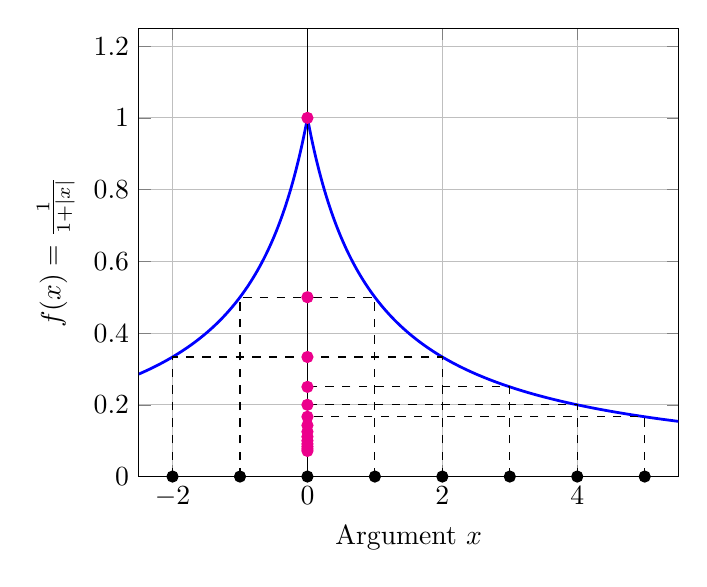
\begin{tikzpicture}
\begin{axis}[
    xlabel={Argument $x$},
    ylabel={$f(x) = \frac{1}{1 + |x|}$},
    xmin=-2.5, xmax=5.5,
    ymin=0, ymax=1.25,
    xmajorgrids,
    ymajorgrids]
\addplot[blue,line width=1pt,domain=-2.5:5.5,samples=801]
    {1 / (1 + abs(x))};
\addplot[black] coordinates { (0,0) (0,1.25)};
\addplot[black, dashed, thin] coordinates {
    (-2,0) (-2,0.3333) (0,0.3333)

    (-1,0) (-1,0.5) (0,0.5)

    (1,0) (1,0.5) (0,0.5)

    (2,0) (2,0.3333) (0,0.3333)

    (3,0) (3,0.25) (0,0.25)

    (4,0) (4,0.2) (0,0.2)

    (5,0) (5,0.1667) (0, 0.1667)};

\addplot[magenta, mark=*] coordinates { (0,1)};
\addplot[magenta, mark=*] coordinates { (0,0.5)};
\addplot[magenta, mark=*] coordinates { (0,0.3333)};
\addplot[magenta, mark=*] coordinates { (0,0.25)};
\addplot[magenta, mark=*] coordinates { (0,0.2)};
\addplot[magenta, mark=*] coordinates { (0,0.1667)};
\addplot[magenta, mark=*] coordinates { (0,0.1428)};
\addplot[magenta, mark=*] coordinates { (0,0.125)};
\addplot[magenta, mark=*] coordinates { (0,0.1111)};
\addplot[magenta, mark=*] coordinates { (0,0.1)};
\addplot[magenta, mark=*] coordinates { (0,0.0909)};
\addplot[magenta, mark=*] coordinates { (0,0.0833)};
\addplot[magenta, mark=*] coordinates { (0,0.0769)};
\addplot[magenta, mark=*] coordinates { (0,0.0714)};

\addplot[black, mark=*] coordinates { (-2,0)};
\addplot[black, mark=*] coordinates { (-1,0)};
\addplot[black, mark=*] coordinates { (0,0)};
\addplot[black, mark=*] coordinates { (1,0)};
\addplot[black, mark=*] coordinates { (2,0)};
\addplot[black, mark=*] coordinates { (3,0)};
\addplot[black, mark=*] coordinates { (4,0)};
\addplot[black, mark=*] coordinates { (5,0)};
\end{axis}
\end{tikzpicture}}
\vspace{-4mm}
\caption{The function $f(x) = \frac{1}{1 + |x|}$ is continuous.
The set of integers $\mathbb{Z}$ is closed.
Yet, the image of this set, $f(\mathbb{Z}) = \{ 1/n : n \in \mathbb{N} \}$, is not closed.
Thus, this is an example of a continuous function along with a set for which $f \left( \overline{\mathbb{Z}} \right) \subsetneq \overline{f \left( \mathbb{Z} \right)}$.}
\end{figure}

\begin{figure}[thb]
\begin{center}
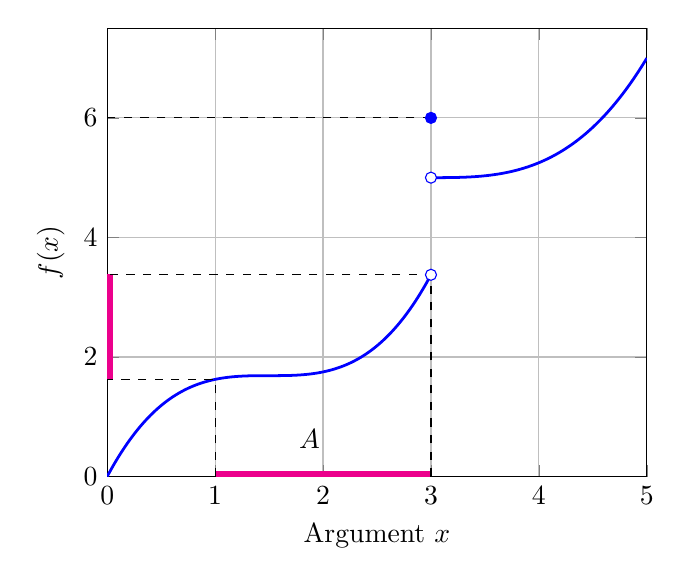
\begin{tikzpicture}
\begin{axis}[
    xlabel={Argument $x$},
    ylabel={$f(x)$},
    xmin=0, xmax=5,
    ymin=0, ymax=7.5,
    xmajorgrids,
    ymajorgrids]
\draw[magenta,fill=magenta] (axis cs:0,1.625) rectangle (axis cs:0.05,3.375);
\draw[magenta,fill=magenta] (axis cs:1,0) rectangle (axis cs:3,0.075);
\addplot[blue,line width=1pt,domain=0:3,samples=201]
    {0.5*(x-1.5)^3 + 1.6875};
\addplot[blue,line width=1pt,domain=3:5,samples=201]
    {0.25*(x-3)^3 + 5};
\addplot[black, dashed] coordinates {
    (1,0) (1,1.625) (0,1.625)

    (3,0) (3,3.375) (0,3.375)

    (3,6) (0,6)};
\addplot[mark=*, draw=blue,fill=white] coordinates {(3, 3.375)};
\addplot[mark=*, draw=blue,fill=white] coordinates {(3,5)};
\addplot[mark=*, draw=blue,fill=blue] coordinates {(3,6)};
\node at (axis cs:1.875,0.625) {$A$};
\end{axis}
\end{tikzpicture}
\end{center}
\vspace*{-8mm}
\caption{Given a function with a discontinuity and a set $A$, the image of the closure, $f \left( \Closure{A} \right)$, need not be a subset of the closure of the image, $\Closure{ f(A) }$, as seen in the example above.}
\end{figure}


\begin{theorem}
Suppose $X$ and $Y$ are two metrizable spaces with metrics $d_X$ and $d_Y$.
Consider a function $f  \colon X \rightarrow Y$.
The function $f$ is continuous if and only if it is $d$-continuous with respect to these metrics.
\end{theorem}
\begin{proof}
Suppose that $f$ is continuous.
For any $x_1 \in X$ and $\epsilon > 0$, let $O_y =  B_{d_Y} (f(x_1), \epsilon)$ and consider the set
\begin{equation*}
O_x = f^{-1} \left( O_y \right)
\end{equation*}
which is open in $X$ and contains the point $x_1$.
Since $O_x$ is open and $x_1 \in O_x$, there exists a $d$-open ball $B_{d_X} (x_1, \delta)$ of radius $\delta>0$ centered at $x_1$ such that $B_{d_X} (x_1, \delta) \subset O_x$.
We also see that $f(x_2) \in O_y$ for any $x_2 \in B_{d_X} (x_1, \delta)$ because $A \subseteq O_x$ implies $f(A) \subseteq O_y$.
It follows that $d_Y \left( f(x_1), f(x_2) \right) < \epsilon$ for all $x_2 \in B_{d_X} (x_1, \delta)$.

Conversely, let $O_y$ be an open set in $Y$ and suppose that the function $f$ is $d$-continuous with respect to $d_X$ and $d_Y$.
For any $x \in f^{-1} (O_y)$, there exists a $d$-open ball $B_{d_Y} (f(x), \epsilon)$ of radius $\epsilon>0$ centered at $f(x)$ that is entirely contained in $O_y$.
By the definition of $d$-continuous, there exits a $d$-open ball $B_{d_X} (x, \delta)$ of radius $\delta>0$ centered at $x$ such that $f \left( B_{d_X} (x,\delta) \right) \subset B_{d_Y} \left( f(x), \epsilon \right)$.
Therefore, every $x \in f^{-1}(O_y)$ has a neighborhood in the same set, and that implies $f^{-1} (O_y)$ is open.
\end{proof}

\begin{definition} \label{definition:SequenceConvergence}
A sequence $x_1, x_2, \ldots$ of points in $X$ is said to \defn{topology}{converge} to $x \in X$ if for every neighborhood $O$ of $x$ there exists a positive integer $N$ such that $x_i \in O$ for all $i \geq N$.
\end{definition}

A sequence need not converge at all.
However, if it converges in a metrizable space, then it converges to only one element.

\begin{theorem}
Suppose that $X$ is a metrizable space, and let $A \subseteq X$.
There exists a sequence of points of $A$ converging to $x$ if and only if $x \in \Closure{A}$.
\end{theorem}
\begin{proof}
Suppose $x_n \rightarrow x$, where $x_n \in A$.
Then, for every open set $O$ containing $x$, there is an $N$, such that $x_n \in O$ for all $n>N$.
By Theorem~\ref{theorem:ClosureConditions}, this implies that $x \in \Closure{A}$.
Let $d$ be a metric for the topology of $X$ and $x$ be a point in $\Closure{A}$.
For each positive integer $n$, consider the neighborhood $B_d \left( x, \frac{1}{n} \right)$.
Since $x\in \Closure{A}$, the set $A \cap B_d \left( x, \frac{1}{n} \right)$ is not empty and we choose $x_n$ to be any point in this set.
It follows that the sequence $x_1, x_2, \ldots$ converges to $x$.
Notice that the ``only if'' proof holds for any topological space, while ``if'' requires a metric.
\end{proof}

\begin{theorem}
\label{theorem:topology_limitpoint_closure}
Let $f \colon X \rightarrow Y$ where $X$ is a metrizable space.
The function $f$ is continuous if and only if for every convergent sequence $x_n \rightarrow x$ in $X$, the sequence $f(x_n)$ converges to $f(x)$.
\end{theorem}
\begin{proof}
Suppose that $f$ is continuous.
Let $O$ be a neighborhood of $f(x)$.
Then $f^{-1}(O)$ is a neighborhood of $x$, and so there exists an integer $N$ such that $x_n \in f^{-1}(O)$ for $n \geq N$.
Thus, $f(x_n) \in O$ for all $n \geq N$ and $f(x_n) \rightarrow f(x)$.

To prove the converse, assume that the convergent sequence condition is true.
Let $A \subseteq X$.
Since $X$ is metrizable, one finds that $x \in \Closure{A}$ implies that there exists a sequence $x_1, x_2, \ldots$ of points of $A$ converging to $x$.
By assumption, $f(x_n) \rightarrow f(x)$.
Since $f(x_n) \in f(A)$, Theorem~\ref{theorem:ContinuityEquivalentConditions} implies that $f(x) \in \Closure{f(A)}$.
Hence $f \left( \Closure{A} \right) \subseteq \Closure{f(A)}$ and $f$ is continuous.
\end{proof}

